\section{Fiasco}

\subsection{Introduction}
The Fiasco kernel is based on the aforementioned L4 specification. Fiasco is a second generation microkernel, which means that it is created with minimalism (nothing exists in the kernel that cannot be moved out of it) and performance in mind. The effect of minimalism can clearly be seen in the number of lines of code the kernel comprises: around 20.000 lines of code for Fiasco compared to around 3.2 million for the Linux kernel. The Fiasco kernel is developed with real-time features in mind, which means that the system is fully preemptable\footnote{Execution can be interrupted at almost any time, which means the work is temporarily halted in favor of (at that moment) higher priority work. After the prioritized work has finished, the system continues with the interrupted execution.}. 

\subsection{History}
DROPS\footnote{Dresden Real-time OPerating Systems project.} \cite{hartig98drops} is a research project which aims to find design techniques to implement a distributed, real-time operating system where every component can guarantee a certain level-of-service to applications. The foundation of DROPS is based on the L4 specification. As the original L4/x86 implementation by Jochen Liedtke had some serious disadvantages (readability, maintainability and licensing issues), the Technische Universit{\"a}t Dresden decided to create their own implementation of the L4 specification, called Fiasco, which could be used by DROPS. Besides implementing the L4.V2 and L4.X2 specifications, Fiasco sets itself apart from other L4 implementations with its real-time features, obviously created with DROPS' real-time focus in mind.\emptyline

Another project related to Fiasco is Fiasco-UX \cite{schonberg01user}, which is a port of the Fiasco microkernel to the Linux system-call interface. This means that Fiasco-UX can be run as an application on a Linux system and due to its special design (no need for kernel-level priviliges) it can even be run as a regular user-level application. One of the main benefits of this approach is its ease of use, particularly when developing applications for Fiasco. Rebooting the machine due to a (kernel) crash is no longer necessary, a simple restart of the Fiasco-UX process suffices. Another advantage is that several instances of Fiasco-UX can run in parallel.\emptyline

We will now discuss in more detail the features of Fiasco that are relevant to our research.

\subsection{Threads}
Besides implementing the L4 thread specification, Fiasco also implements some additional mechanisms for performance- and real-time support purposes. Some of the performance optimizations stem from \cite{liedtke93improve}.

\subsubsection{Scheduling}
As the L4 specification dictates, a thread has properties such as a time quantum and priority associated with it; these properties of a thread are called its \emph{scheduling context} and are used in the scheduling of threads. To support the real-time features of Fiasco, each thread can also have an additional real-time scheduling context\footnote{This is not part of the L4 specification.}. An \emph{execution context} is a runnable, schedulable thread. At all times there is only one active execution context (or thread), as Fiasco does not support multi-processor execution (it will only use one of the processors available). A thread's current state of execution is stored in its thread control block (TCB), which resides in the kernel. Switching execution of threads can therefore be done through a simple TCB switch. The scheduler uses the \emph{ready-list} (containing all threads ready to be run) to decide what thread to run next. More details on scheduling in Fiasco can be found in \cite{steinberg05quality}.

\subsubsection{Ready-list}
As said, the system keeps a list of all threads ready to be executed: the ready-list. Although it might seem odd at first, the ready-list can contain threads that are \textit{not} ready to be executed. If the scheduler finds such a thread while traversing the ready-list, it is immediately removed from it. The goal of this \emph{lazy-scheduling} is improving the performance of IPC. As an example, we look at a call to the \emph{call} IPC function, in which a sender sends a message to a receiver and then waits for that receiver to send a message back. If we were to strictly adhere to the property that the ready-list only contains ready threads, this IPC call would result in the following modifications to the ready-list:

\begin{itemize}
 \item After the sender has sent its message, the sender enters a waiting mode and has to be dequeued.
 \item After the sender has sent its message, the receiver becomes ready and has to be enqueued.
 \item After the receiver has sent its message, the receiver enters a waiting mode and has to be dequeued.
 \item After the receiver has sent its message, the sender becomes ready and has to be enqueued.
\end{itemize}

We see that this common scenario results in four different changes to the ready-list. Obviously, this is detremental to IPC performance. However, if we allow non-ready threads in the ready-list and exclude the current executing thread from it (which is ready by definition), all four modifications can be saved. After the sender has sent its message, the receiver does not need to be enqueued as it has become the current executing thread. Similarly, once the receiver has sent its message back, the sender does not need to be enqueued as it will be the currently executing thread. Both dequeue actions can be saved as we allow threads in the ready-list that are not ready, which is precisely what entering a waiting mode signifies. To successfully apply this lazy-scheduling, the kernel has to make sure that the current executing thread will be enqueued in the ready-list if it cannot finish its task within its timeslice. If we would leave out this clause, the current executing thread is not guaranteed to get scheduled again (remember that it is not contained in the ready-list while executing), which is necessary in order to finish its task.\emptyline

To switch execution from sender to receiver (and vice versa) without ready-list scheduling, the system uses their execution contexts. Say we want to switch execution from thread A (which is the current active thread) to thread B, but without using the ready-list. To do so, a simple switch of execution context from A to B suffices, as the current execution context determines what is executed. It is not necessary to also switch the scheduling context from A to B, in fact it is better not to for the following reason. If the scheduling context is not changed when the execution context is switched, thread B gets to execute as if it were A, which means that it can execute for the remainder of A's timeslice. This optimization gives B more execution time than it would normally have, thereby allowing it to finish sooner. In our \emph{call} example, this means that after the sender has sent its message, an execution switch is made to the receiver which gets to execute in the sender's timeslice. Therefore, it is likely that the receiver is able to send a message back sooner, as the sender's timeslice remainder would otherwise be wasted by waiting on the receiver.\emptyline

In some situations, it might not be useful to immediately switch to the receiver but instead enqueue the receiver in the ready-list (which is the normal way in which a thread gets to execute). For this situation the \emph{deceit-bit hack} can be used. Originally, the deceit-bit was used in the L4 clans \& chiefs concept, but as this concept proved too inflexible it is almost never implemented. Therefore, the deceit-bit was \textit{free} for other purposes and in Fiasco it is used to signal that no lazy-scheduling should be applied.

\subsection{Synchronization}
Having a fully preemptable system requires some form of synchronization for critical parts. Fiasco supports two different types of synchronization: \emph{lock-free}- and \emph{wait-free} synchronization. The main difference between the two synchronization types is in their intended use: lock-free synchronization should be used for time-critical synchronization (such as the synchronizing of frequently accessed, global data) and wait-free synchronization should be used for non time-critical operations (such as the synchronizing of local data). The two synchronization types are implemented as follows:

\begin{itemize}
	\item Lock-free synchronization: this is achieved through atomic updating of memory\footnote{The x86 processor provides the compare-and-swap (CAS) instruction for exactly this purpose.}. It tries to exchange old data for new data and if this fails it simply retries. In order to prevent the system from retrying infinitely (which would invalidate the real-time properties of the system), a specific retry-count can be set. While setting the data, interrupts will be temporarily disabled to prevent another thread from modifying the data.
	\item Wait-free synchronization: this is a locking-type of synchronization, in which exclusive access to resources can be obtained by creating a lock. Fiasco expands on this well-known mechanism by introducing \emph{switch locks} (also referred to as \emph{helping locks}). Suppose thread A has locked a resource X which thread B also wants to access. Normally, B would just use up all of its execution time waiting on A to release the lock on X. However, instead of wasting execution time on waiting, B can also help A release its lock sooner by donating its remaining timeslice to A. Now A has more execution time available and will likely release the lock on X sooner, which is exactly what B wants. One might note the similarity of this optimization to the thread switch optimization in the ready-list description.
\end{itemize}

A full description of the design philosophy and implementation of these two synchronization mechanisms can be found in \cite{hohmuth01pragmatic}.

\subsection{Locks}
Wait-free synchronization in Fiasco can be achieved through the use of locks. Basically there are two types of locks: regular- and switch locks. Of the former there exists just one in Fiasco, namely the CPU lock, which temporarily disables interrupts. This lock should only be used for very short intervals as it can negatively influence the real-time features of the system. The other two locks in Fiasco are switch locks. The first switch lock is the thread lock, which locks access to a thread. The second switch lock is the helping lock, which is similar to the switch lock save from the fact that it also works when the scheduling system has not yet been loaded.\emptyline

Switch locks are designed explicitly with IPC performance in mind; its basic optimization principle strongly resembles that discussed in the ready-list discussion. The implementation is as follows. When the current thread tries to acquire a lock on a resource by using a switch lock but detects that the resource is already locked, the lock count of the current thread is incremented. After incrementing the lock count, the switch lock keeps on switching to the lock owner (by switching the execution context to that of the lock owner) until the lock is free and can be acquired. Afterwards, when the lock is released, the lock count is decremented and the lock checks if it has been helped by another thread (which donated execution time to the thread holding the lock), if so it switches the execution context to that of the helper.\emptyline

When a thread is locked, it will not be selected by the scheduler. Should a switch be made to a locked thread, the system will immediately switch to that thread's lock owner. Although locked threads normally do not get scheduled, an exception arises when a thread is killed. A thread that is to be killed should hold no locks at all, therefore the system keeps scheduling such a thread until it has released all its locks. The thread's lock count is used to determine if any locks are still present.

\subsection{Timeouts}
Fiasco recognizes three different types of timeouts: IPC-, deadline- and timeslice timeouts. An IPC timeout is used to restrict an IPC call to a specific maximum time, which can be used to prevent senders and receivers from waiting endlessly on each other. A deadline timeout is used to set timed deadlines and a timeslice timeout is used to signal the end of a timeslice.\emptyline

Internally, timeouts are stored in a list that is ordered in ascending timeout order (the head of the list is the oldest timeout and the first to occur). When the system checks if timeouts occured, the timeout list can thus be traversed sequentially. Therefore, detecting timeouts is very fast whereas enqueuing or dequeuing is rather slow. For more details on the implementation of timeouts see \cite{reusner05impl}.

\subsection{IPC}
IPC in Fiasco supports all L4 IPC calls, namely \emph{send}, \emph{receive}, \emph{wait}, \emph{reply-wait} and \emph{call}. All these functions are internally supported through one generic function: \emph{sys\_ipc()}, which parameters determine the actual call made. We will now describe the general setup of IPC in Fiasco.

\subsubsection{Sender and receiver roles}
IPC in Fiasco is synchronous and thus always involves a single sender- and receiver communicating (sending messages) with each other. In Fiasco, there are separate definitions for the sender- and receiver roles. As threads need to both send- \textit{and} receive messages, they extend (inherit from) both the receiver- and the sender role. In Fiasco, only threads extend the receiver role, in other words only threads can receive IPC messages. However, there are two more objects extending the sender role, namely the IRQ and preemption objects. The first translates hardware interrupts into IPC messages, which demonstrates the very generic applicability of Fiasco's receiver/sender setup. The second sends messages dealing with preemptions. As both the IRQ and preemption objects can only send messages (as they do not extend the receiver role), they are also known as \emph{passive senders}.\emptyline

\begin{figure}[ht]
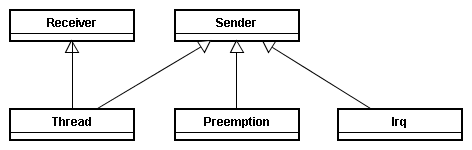
\includegraphics[scale=0.50]{images/diagrams/ipc_class_ipc_roles}
\caption{Fiasco IPC roles diagram.}
\end{figure}

Due to IPC's synchronous nature, a receiver can only receive a message from a single sender. As it is possible that a receiver is unable to directly engage in IPC with a sender (for example because it is already engaged in IPC with another sender), the receiver should be able to queue send requests. This is achieved in Fiasco by letting the receiver have a sender list, which is a list of senders wanting to send a message to the receiver. Once a receiver engages in IPC with a sender, that sender is removed from the sender list (if he was it in).\emptyline

When an IPC call is made, the transferring of a message is handled from the viewpoint of the sender, it is the sender that determines which actions to do first and how to continue. An exception to this situation occurs when the sender is a passive sender; in this case the receiver controls IPC.

\subsubsection{IPC overview}
Although there are five different IPC calls, internally there is only one function that handles IPC: \emph{sys\_ipc()}. IPC (and thus the \emph{sys\_ipc()} function) can be divided into a send and receive part. Obviously, the send part handles the sending of an IPC message and the receive part handles the receiving thereof. The table below lists what IPC parts are involved in the five IPC calls:

\begin{table}[ht]
\begin{tabular}{l|l|p{20em}}
IPC call & Send part & Receive part \\
\hline
\emph{send} & x & - \\
\emph{receive} & - & x \\
\emph{wait} & - & x \\
\emph{reply-wait} & x & x \\
\emph{call} & x & x \\
\end{tabular}
\caption{Mapping of L4 IPC calls to Fiasco send and receive parts.}
\end{table}

The following schema gives an overview of how the send and receive parts are handled in Fiasco:

\begin{figure}[ht]
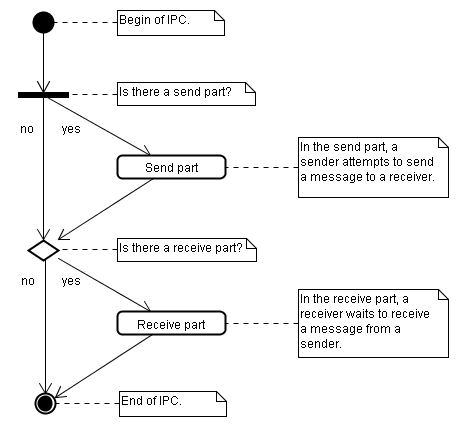
\includegraphics[scale=0.50]{images/diagrams/ipc_activity_ipc_overview}
\caption{IPC overview.}
\end{figure}

One might remember that in the \emph{reply-wait} and \emph{call} calls, the message sending preceded the receiving of a message. In Fiasco, the receive part is handled \textit{after} the send part to allow the aforementioned two calls to be handled in a single execution of the IPC path (this sequential structure has no influence on the functionality of the other three IPC calls).\emptyline

Before a message can be sent in the send part, the sender and receiver have to agree upon engaging in IPC; this is referred to as the \emph{handshake}. It is possible that the receiver is not immediately ready to receive a message from the sender, for example because it is still engaged in IPC with another sender; in that case the sender is added to the receiver's sender list and waits for the receiver to become ready. If an error occured in the handshake, IPC is aborted. However, if the handshake was successful, the sender can then send its message to the receiver. The following schema displays this set-up:

\begin{figure}[!ht]
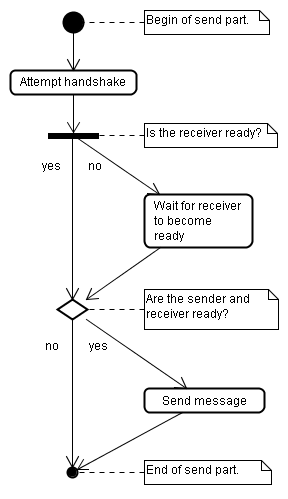
\includegraphics[scale=0.50]{images/diagrams/ipc_activity_send_part}
\caption{IPC send part overview.}
\end{figure}

As control of IPC is mostly handled by the sender (and thus in the send part), the receive part does relatively little. What \textit{is} done in the receive part is that the receiver enters a loop. With each iteration, it checks if it is ready to receive a message and if there is a sender that wants to send a message (which is indicated by a non-empty sender list). If there is such a sender, the receiver sends it a signal to indicate that it is ready to receive a message. That sender is subsequently removed from the sender list by the receiver. Only when the receiver is not ready to receive a message is the receive part aborted.

\begin{figure}[!ht]
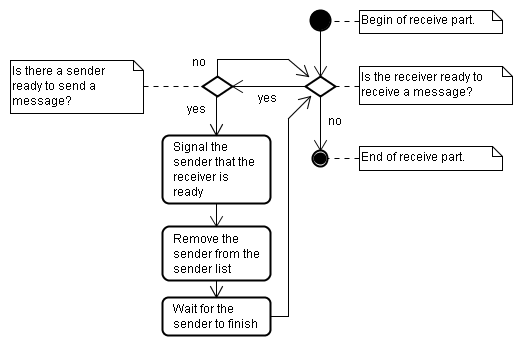
\includegraphics[scale=0.50]{images/diagrams/ipc_activity_receive_part}
\caption{IPC receive part overview.}
\end{figure}

\subsubsection{IPC paths}
Because IPC in Fiasco is unbuffered, no messages are temporarily stored by the kernel; instead messages are transferred directly between sender and receiver. As described in the L4 specification, Fiasco discerns between three different message types: untyped data (direct strings), memory-buffer references (indirect strings) and memory mappings (flexpages).\emptyline

There are two paths in Fiasco through which an IPC message can be transferred: a short- and long IPC path. 
\begin{itemize}
  \item Short IPC path: this path uses only the system registers for transferring messages. The size of the data which can be transferred is thus limited to the size of the available registers. The advantages of only using the system registers for message transfer are that it is very fast and that no page-faults can occur (as no user-space memory is accessed). As an example of where the short IPC path is put to good use, when a page-fault IPC message is sent to a pager, that pager should respond with a flexpage IPC message to resolve the page-fault. Because a single flexpage does not exceed the size of the registers, it can be sent using the short IPC path allowing for a fast response by the pager. Secondly, when a direct string is sent, the system puts as much of that direct string into the registers; if the direct string does nog fit completely into the registers, the rest of the direct string is transferred using the long IPC path.
  \item Long IPC path: all message types can be transferred through the long IPC path, that includes indirect strings. Where the short IPC path limits the sending of flexpages to a single value, the long IPC path can send several flexpages at once. The transferring of messages is done by creating an IPC window. The IPC window is a part of the receiver's address space, which is mapped to the sender's address space during the message transfer. The sender can now directly copy the messages into the address space of the receiver, which prevents the kernel from buffering the messages. The main disadvantage of long IPC is that it has to invoke user-space memory, which could generate page-faults. A generated page-fault is sent to the pager of the receiver, as it is the receiver's address space that is being written to. Also, the long IPC path is slower than the short IPC path.
\end{itemize}

\subsubsection{IPC shortcut path}
Besides the two aforementioned IPC paths, there is also an IPC shortcut path. Basically, the IPC shortcut is an alternative version of the short IPC path (it thus also transfers messages through the system registers), but with some further restrictions applied to it (which enable performance optimizations). One of the restrictions of the shortcut is that it does not support the receive- and wait calls. Another restriction is that a single flexpage cannot be sent using the shortcut, only direct strings which fit into the registers are thus eligible for use with the IPC shortcut. Furthermore, the supported timeouts are limited to zero- (immediate response required) and infinite (no time-out at all) timeouts. The IPC shortcut completely runs with interrupts disabled. \emptyline

The reason why the IPC shortcut was developed is simple: most of the system calls are IPC calls and most of the IPC messages are short IPC messages. Therefore, when the transfer of these short messages is optimized, the performance of the whole system is likely to improve significantly. There are two different versions of the shortcut. The normal version is implemented in C++, but there is also an optimized version of the shortcut, which is written in assembler and has been developed by Michael Peter \cite{peter02leistung}.

\subsubsection{IPC states}
The state of an IPC operation is stored at the receiver; this state is stored as a bit mask in which each bit corresponds to a specific state the thread can be in (for example waiting for a receiver or sending an IPC message). There are several functions to modify the state, which can add-, delete- or at once add- and delete bits in the state. These functions are respectively \emph{state\_add()}, \emph{state\_del()} and \emph{state\_change()}. All these functions are atomic operations, which means that they are guaranteed to succeed. The disadvantage of these atomic operations is that they are unnecessarily expensive when interrupts are already disabled. In this case regular operations would have exactly the same result as they too are then guaranteed to succeed, but without incurring the performance penalty of atomic operations. Fiasco therefore offers non-atomic variants of the state modification functions which are suffixed with "\_dirty" (leading to the \emph{state\_add\_dirty()}, \emph{state\_del\_dirty()} and \emph{state\_change\_dirty()} functions). Please note that these \textit{dirty} functions assume that interrupts are disabled, they do not check this themselves; it is therefore the responsibility of the caller to make sure interrupts are disabled when calling these functions.

\subsubsection{Priority inversion}
One of the classic scheduling problems is priority inversion, where a lower priority task is prioritized over a higher priority task. This situation occurs when a lower priority task has locked a shared resource that a higher priority task also wants to access. The higher priority task has no choice but to wait for the lower priority task to release the lock; the priorities are thus temporarily inversed. In Fiasco's old IPC path this problem existed when a combined send- and wait call was made. Let us consider a situation in which a sender A is engaged in a combined send- and wait operation with receiver B. As soon as A has sent its message to B, sender A enters a waiting state and an immediate execution context switch is made to receiver B (this optimization is described in the ready-list section). Because the receiver B gets to execute in the scheduling context of A, it will temporarily inherit the priority of A. Now suppose just before the switch to B, a second sender (which we call C) tries to send a message to B. If the priority of C is less than or equal to the priority of A, there is no problem. However, when C has a higher priority than B, the switch from B to A (which has B's priority) violates the priority-based scheduling invariant\footnote{Which states that higher priority threads should always be scheduled before lower priority threads.}.\emptyline

This problem was fixed in the current IPC implementation; its solution was actually quite simple: before switching to the receiver, the sender should check if there is a sender with a higher priority than its own that wants to send a message to the same receiver. Should this be the case, the receiver is added to the ready-list and the system switches to the higher priority sender. If no other higher priority sender exists, the immediate switch to the receiver can be done without any problem.

\subsubsection{Real-time features}
Because IPC is of vital importance to the performance of Fiasco (in fact, it is of vital performance to \textit{any} microkernel), improving IPC is thus one of the key performance improving strategies. However, with Fiasco a constant eye has to kept at the real-time features of the system. Often, there is a trade-off between performance and real-time support. This can clearly be seen in Ren\'e Reusner's attempt to improve the performance of IPC in Fiasco, which includes clear graphs detailing the trade-off results \cite{reusner05impl}.\emptyline

Probably the best example of such a performance versus real-time features trade-off is the decision on which parts of the IPC path should be non-interruptible. If one makes the IPC path non-interruptible, this prevents the use of synchronization mechanisms, which are required in an interruptible path and thus improves performance. The real-time features are invalidated though. The current IPC path is non-interruptible in the following phases: the setup, rendez-vous and finish phase. Furthermore, when sending direct strings in the register transfer (short IPC) phase, the system remains non-interruptible. However, when a flexpage is sent in the register transfer phase or the memory transfer phase is used, the system \textit{is} interruptible. An interruptible path has good real-time features, but this comes at the cost of decreased performance.\emptyline

Although most phases are non-interruptible, in- and between phases interrupt points and -regions have been inserted to preserve the real-time features. An interrupt region is created by calling \emph{Proc::sti()} (enable interrupts) at the beginning- and \emph{Proc::cli()} (disable interrupts) at the end of the region. An interrupt point is created by calling the \emph{Proc::preemption\_point()} function\footnote{Internally, this function first enables interrupts by calling \emph{Proc::sti()}, than executes the \emph{nop()} instruction (which does not do anything) twice to give interrupts the chance and then disables interrupts again by calling \emph{Proc::cli()} after which it returns.}. Please note that there also is a preemption point at the very beginning of an IPC operation, before the \emph{sys\_ipc()} function is called. The disadvantage of using interrupt points and -regions is that additional checks are needed because the state might have changed while interrupts were allowed.

\begin{figure}[ht]
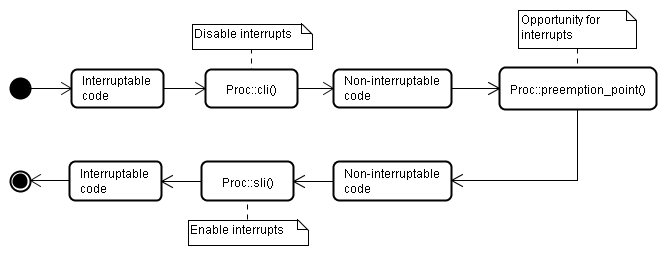
\includegraphics[scale=0.50]{images/diagrams/ipc_activity_interrupts}
\caption{Fiasco interrupt transitions.}
\end{figure}